\documentclass[conference]{IEEEtran}
\IEEEoverridecommandlockouts
\usepackage{cite}
\usepackage{amsmath,amssymb,amsfonts}
\usepackage{graphicx}
\usepackage{booktabs}
\usepackage[hidelinks]{hyperref}
\usepackage{etoolbox}
% "Abstract:" and "Index Terms:" instead of the class's em dash
\makeatletter
\def\hera@nodash#1{\loop\patchcmd{#1}{---}{:\ }{\let\hera@more\iftrue}{\let\hera@more\iffalse}\hera@more\repeat}
\hera@nodash\abstract \hera@nodash\IEEEkeywords
\makeatother
% Auto-generated by experiments/make_tables.py -- do not edit
\newcommand{\apprCloud}{85.3}
\newcommand{\apprEdge}{87.4}
\newcommand{\apprHera}{76.7}
\newcommand{\apprHeraFixed}{87.5}
\newcommand{\apprHeraNoA}{76.6}
\newcommand{\apprHeraNoDT}{83.8}
\newcommand{\apprHeraNoUQ}{19.2}
\newcommand{\apprPoint}{26.4}
\newcommand{\apprRandom}{83.2}
\newcommand{\apprScore}{78.8}
\newcommand{\apprWidth}{76.6}
\newcommand{\bestRmse}{1047}
\newcommand{\bestRmseModel}{TCN+DT}
\newcommand{\bytesCloud}{112.0}
\newcommand{\bytesEdge}{0.0}
\newcommand{\bytesHera}{116.6}
\newcommand{\bytesHeraFixed}{27.2}
\newcommand{\bytesHeraNoA}{116.5}
\newcommand{\bytesHeraNoDT}{116.6}
\newcommand{\bytesHeraNoUQ}{69.3}
\newcommand{\bytesPoint}{112.0}
\newcommand{\bytesRandom}{124.0}
\newcommand{\bytesScore}{117.0}
\newcommand{\bytesWidth}{116.5}
\newcommand{\cceCloud}{0.062}
\newcommand{\cceCloudNoDT}{0.044}
\newcommand{\cceEdge}{0.054}
\newcommand{\cloudLat}{0.24}
\newcommand{\cloudMacs}{0.55M}
\newcommand{\cloudModel}{CNN-LSTM}
\newcommand{\cloudParams}{15.7k}
\newcommand{\commReduction}{-4}
\newcommand{\covMinCloud}{0.20}
\newcommand{\covMinCloudNoDT}{0.34}
\newcommand{\covMinEdge}{0.13}
\newcommand{\cqrCovMax}{0.89}
\newcommand{\cqrCovMin}{0.83}
\newcommand{\detAnomAuroc}{0.81}
\newcommand{\detAnomFone}{0.27}
\newcommand{\detAnomPrecision}{0.27}
\newcommand{\detAnomRecall}{0.26}
\newcommand{\detCloudLBAuroc}{0.67}
\newcommand{\detCloudLBFone}{0.13}
\newcommand{\detCloudLBPrecision}{0.07}
\newcommand{\detCloudLBRecall}{0.64}
\newcommand{\detEdgeLBAuroc}{0.69}
\newcommand{\detEdgeLBFone}{0.16}
\newcommand{\detEdgeLBPrecision}{0.10}
\newcommand{\detEdgeLBRecall}{0.52}
\newcommand{\detIsoAuroc}{0.77}
\newcommand{\detIsoFone}{0.19}
\newcommand{\detIsoPrecision}{0.27}
\newcommand{\detIsoRecall}{0.15}
\newcommand{\edgeLat}{0.13}
\newcommand{\edgeMacs}{34k}
\newcommand{\edgeModel}{Edge-GRU}
\newcommand{\edgeParams}{2.5k}
\newcommand{\escAlphaFifty}{64.8}
\newcommand{\escAlphaFive}{98.7}
\newcommand{\escAlphaThirty}{74.1}
\newcommand{\escCloud}{100.0}
\newcommand{\escEdge}{0.0}
\newcommand{\escHera}{87.5}
\newcommand{\escHeraFixed}{3.9}
\newcommand{\escHeraNoA}{87.4}
\newcommand{\escHeraNoDT}{87.5}
\newcommand{\escHeraNoUQ}{32.7}
\newcommand{\escPoint}{100.0}
\newcommand{\escRandom}{85.2}
\newcommand{\escScore}{88.9}
\newcommand{\escWidth}{87.4}
\newcommand{\fmAlphaFifty}{56.6}
\newcommand{\fmAlphaFive}{83.6}
\newcommand{\fmAlphaThirty}{65.0}
\newcommand{\fmCloud}{84.0}
\newcommand{\fmEdge}{86.8}
\newcommand{\fmHera}{75.0}
\newcommand{\fmHeraFixed}{86.8}
\newcommand{\fmHeraNoA}{75.0}
\newcommand{\fmHeraNoDT}{82.6}
\newcommand{\fmHeraNoUQ}{17.0}
\newcommand{\fmPoint}{23.6}
\newcommand{\fmRandom}{81.8}
\newcommand{\fmScore}{77.0}
\newcommand{\fmWidth}{75.0}
\newcommand{\furgCloud}{36.6}
\newcommand{\furgEdge}{21.9}
\newcommand{\furgHera}{35.0}
\newcommand{\furgHeraFixed}{22.0}
\newcommand{\furgHeraNoA}{35.0}
\newcommand{\furgHeraNoDT}{42.7}
\newcommand{\furgHeraNoUQ}{5.2}
\newcommand{\furgPoint}{5.7}
\newcommand{\furgRandom}{32.8}
\newcommand{\furgScore}{35.6}
\newcommand{\furgWidth}{35.0}
\newcommand{\kmacsCloud}{551}
\newcommand{\kmacsEdge}{34}
\newcommand{\kmacsHera}{516}
\newcommand{\kmacsHeraFixed}{56}
\newcommand{\kmacsHeraNoA}{516}
\newcommand{\kmacsHeraNoDT}{516}
\newcommand{\kmacsHeraNoUQ}{214}
\newcommand{\kmacsPoint}{551}
\newcommand{\kmacsRandom}{504}
\newcommand{\kmacsScore}{525}
\newcommand{\kmacsWidth}{516}
\newcommand{\latCloud}{50.2}
\newcommand{\latEdge}{0.1}
\newcommand{\latHera}{44.1}
\newcommand{\latHeraFixed}{2.1}
\newcommand{\latHeraNoA}{44.0}
\newcommand{\latHeraNoDT}{44.1}
\newcommand{\latHeraNoUQ}{16.5}
\newcommand{\latPoint}{50.2}
\newcommand{\latRandom}{42.9}
\newcommand{\latScore}{44.8}
\newcommand{\latWidth}{44.0}
\newcommand{\lowMissCritCloud}{42}
\newcommand{\lowMissCritCloudNoDT}{40}
\newcommand{\lowMissCritEdge}{52}
\newcommand{\macsReduction}{6}
\newcommand{\maeCloud}{717}
\newcommand{\maeCloudNoDT}{676}
\newcommand{\maeEdge}{525}
\newcommand{\missUrgCloud}{35.9}
\newcommand{\missUrgEdge}{47.5}
\newcommand{\missUrgHera}{35.9}
\newcommand{\missUrgHeraFixed}{47.1}
\newcommand{\missUrgHeraNoA}{36.1}
\newcommand{\missUrgHeraNoDT}{32.5}
\newcommand{\missUrgHeraNoUQ}{77.0}
\newcommand{\missUrgPoint}{76.5}
\newcommand{\missUrgRandom}{38.6}
\newcommand{\missUrgScore}{36.0}
\newcommand{\missUrgWidth}{36.1}
\newcommand{\mpiwAsymCloud}{1918}
\newcommand{\mpiwAsymCloudNoDT}{1928}
\newcommand{\mpiwAsymEdge}{1959}
\newcommand{\mpiwCloud}{2008}
\newcommand{\mpiwCloudNoDT}{2147}
\newcommand{\mpiwEdge}{1879}
\newcommand{\nBearingsCovLow}{11}
\newcommand{\nzFmHeraPoint}{17}
\newcommand{\nzHeraCloud}{4}
\newcommand{\nzHeraPoint}{14}
\newcommand{\nzHeraWidth}{2}
\newcommand{\pFmHeraPoint}{$<$0.001}
\newcommand{\pHeraCloud}{n/a}
\newcommand{\pHeraPoint}{$<$0.001}
\newcommand{\pHeraWidth}{n/a}
\newcommand{\picpAsymCloud}{0.84}
\newcommand{\picpAsymCloudNoDT}{0.82}
\newcommand{\picpAsymEdge}{0.83}
\newcommand{\picpCloud}{0.85}
\newcommand{\picpCloudNoDT}{0.83}
\newcommand{\picpEdge}{0.84}
\newcommand{\rawCovMax}{0.69}
\newcommand{\rawCovMin}{0.31}
\newcommand{\rawpicpCloud}{0.36}
\newcommand{\rawpicpCloudNoDT}{0.47}
\newcommand{\rawpicpEdge}{0.69}
\newcommand{\rmseCloud}{1093}
\newcommand{\rmseCloudNoDT}{1096}
\newcommand{\rmseEdge}{816}
\newcommand{\rmsePolCloud}{1090}
\newcommand{\rmsePolEdge}{809}
\newcommand{\rmsePolHera}{1083}
\newcommand{\rmsePolHeraFixed}{811}
\newcommand{\rmsePolHeraNoA}{1084}
\newcommand{\rmsePolHeraNoDT}{1088}
\newcommand{\rmsePolHeraNoUQ}{1014}
\newcommand{\rmsePolPoint}{1100}
\newcommand{\rmsePolRandom}{1059}
\newcommand{\rmsePolScore}{1086}
\newcommand{\rmsePolWidth}{1084}
\newcommand{\rttMs}{50}
\newcommand{\shapAdditivity}{154.8}
\newcommand{\tauAmax}{18.4}
\newcommand{\tauAmin}{17.0}
\newcommand{\unsafeAlphaFifty}{19.0}
\newcommand{\unsafeAlphaFive}{5.4}
\newcommand{\unsafeAlphaThirty}{14.1}
\newcommand{\unsafeCloud}{5.4}
\newcommand{\unsafeEdge}{6.7}
\newcommand{\unsafeHera}{9.4}
\newcommand{\unsafeHeraFixed}{6.7}
\newcommand{\unsafeHeraNoA}{9.6}
\newcommand{\unsafeHeraNoDT}{6.5}
\newcommand{\unsafeHeraNoUQ}{48.2}
\newcommand{\unsafePoint}{41.0}
\newcommand{\unsafeRandom}{6.1}
\newcommand{\unsafeScore}{7.6}
\newcommand{\unsafeWidth}{9.5}

\newcommand{\Hc}{H_{\mathrm{c}}}
\newcommand{\Hp}{H_{\mathrm{p}}}
\graphicspath{{../paper/}}

\begin{document}

\title{HERA-PdM: A Reference Architecture for Uncertainty-Gated, Human-Approved Predictive Maintenance in Industry~5.0}

\author{\IEEEauthorblockN{Pradeep Somasundaram}}

\maketitle

\begin{abstract}
This design paper proposes HERA-PdM, a reference architecture for hierarchical predictive maintenance (PdM) in human-centric Industry~5.0 plants. Four software agents (edge monitoring, Digital Twin state, fog/cloud prognostics and maintenance decision) exchange explicit messages; every remaining-useful-life (RUL) estimate carries a conformally calibrated interval; the edge escalates to higher tiers only when its interval cannot fix a maintenance action; and schedule/urgent actions are issued as explained recommendations that require human approval. We specify the agents, message schemas, decision rules and the safety property the escalation rule provides, describe how the architecture maps onto a production line through an explicitly hypothetical deployment scenario, and summarize preliminary evidence from a companion empirical study on two public bearing datasets, which shows when the design is expected to help and when it is not. We close with the open problems that a deployment would have to solve, notably bearing-level alarm-timing guarantees and operator workload.
\end{abstract}

\begin{IEEEkeywords}
predictive maintenance, reference architecture, conformal prediction, edge computing, Digital Twin, human-in-the-loop, Industry 5.0
\end{IEEEkeywords}

\section{Motivation and Design Goals}
Predictive maintenance aims to intervene before failure using condition data~\cite{lei2018machinery}. In plants moving towards Industry~5.0, three constraints shape any PdM system: sensing happens at the machine and bandwidth to central servers is limited~\cite{ren2021cloudedge}; predictions must state how far they can be trusted~\cite{basora2025benchmark,javanmardi2023conformal}; and humans remain responsible for consequential actions~\cite{xu2021industry5}, while decision-makers often do not adopt opaque advice~\cite{vanoudenhoven2023pdm5}. Hierarchical and agentic PdM systems exist~\cite{saleh2026hama,mendonca2026human,coulibaly2026masdt}, but they escalate on anomaly thresholds or uncalibrated confidence~\cite{saleh2026hama,yao2026ecdistill}. HERA-PdM is designed around five goals:
\begin{enumerate}
\item[G1] \emph{Local by default:} routine monitoring runs on the machine.
\item[G2] \emph{Calibrated uncertainty everywhere:} every RUL estimate is an interval with a stated coverage level~\cite{romano2019cqr,barber2021jackknife}.
\item[G3] \emph{Decision-driven escalation:} computation moves up only when the local estimate cannot decide the maintenance action.
\item[G4] \emph{Human authority:} high-impact actions are recommendations with evidence, never automatic.
\item[G5] \emph{Auditability:} all numbers in a recommendation are traceable to a validated predictor; no generative model produces quantitative content.
\end{enumerate}

\section{Architecture}
\begin{figure}[t]
\centering
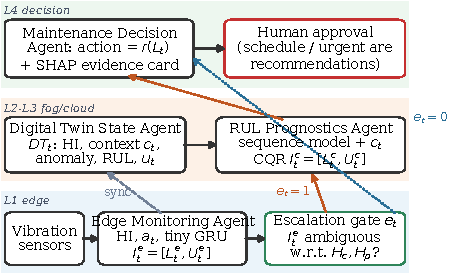
\includegraphics[width=\columnwidth]{figures/fig1_architecture.pdf}
\caption{HERA-PdM reference architecture: agents, tiers and messages.}
\label{fig:arch}
\end{figure}

Fig.~\ref{fig:arch} shows the tiers. Table~\ref{tab:agents} lists each agent's inputs, outputs and message.

\begin{table}[t]
\centering
\caption{Agents and message interfaces.}
\label{tab:agents}
\footnotesize\setlength{\tabcolsep}{2pt}
\begin{tabular}{p{1.55cm}p{3.15cm}p{3.0cm}}
\toprule
Agent (tier) & Responsibility & Message out \\
\midrule
Edge Monitoring (L1) & features $x_t$, health index $h_t$, anomaly $a_t$, tiny quantile model, calibrated $I^e_t$, gate $e_t$ & sync $(t,h_t,a_t)$ each snapshot; window on $e_t{=}1$ \\
Digital Twin State (L2) & synchronized record $DT_t$, degradation context $c_t$ & $c_t$ to prognostics; state history \\
RUL Prognostics (L3) & sequence model on window $+\,c_t$, calibrated $I^c_t$ & $(\hat R_t, I^c_t)$ \\
Maintenance Decision (L4) & action $r(L_t)$, SHAP evidence, card & recommendation; approval request \\
Human operator & approve / reject / defer & decision log (audit) \\
\bottomrule
\end{tabular}
\end{table}

\textit{Uncertainty layer.} Each tier outputs quantiles that are conformalized; with cross-fitting (CV+~\cite{barber2021jackknife}) all historical assets serve as calibration data. The action of an interval is $r(L_t)$ with regions \textsc{urgent} ($\le\Hc$), \textsc{schedule} ($\le\Hp$) and \textsc{continue}.

\textit{Escalation rule.} The edge escalates when $I^e_t=[L^e_t,U^e_t]$ straddles a boundary in $\{\Hc,\Hp\}$ or when anomaly evidence contradicts a \textsc{continue} verdict. A locally resolved \textsc{continue} requires $L^e_t>\Hp$, so a critical asset is left running at the edge only when the true RUL lies outside the calibrated interval:
\begin{equation}
\Pr(e_t{=}0,\ \pi_t{=}\textsc{continue},\ y_t\le\Hc)\le\Pr(y_t\notin I^e_t).
\end{equation}

\textit{Human-in-the-loop.} The decision agent emits a card with predicted RUL, interval, anomaly evidence, top SHAP~\cite{lundberg2017shap} contributors and a templated rationale; \textsc{schedule}/\textsc{urgent} wait for approval, and approvals are logged.

\section{Illustrative Deployment Scenario (Hypothetical)}
\emph{This section is a design walk-through. All quantities in it are assumptions chosen for illustration; none is a measurement.}

Consider a hypothetical packaging line with conveyor drive bearings instrumented with two-axis accelerometers. An edge node per machine extracts features each snapshot and keeps only the healthy baseline and a short window. While intervals stay inside the \textsc{continue} region the node sends only the 12-byte sync message, which the fog-level Digital Twin uses to maintain long-horizon context. When a bearing's edge interval begins to straddle $\Hp$, the node streams its feature window to the fog prognostics agent, whose interval and SHAP evidence populate a card routed to the shift maintenance planner. The planner approves a scheduled replacement for the next planned stop; an urgent recommendation would additionally notify the line supervisor. In such a deployment, $\Hc$ and $\Hp$ would be set from the plant's spare-part lead time and planned-stop calendar, and the calibration set would be refreshed as new run-to-failure histories accumulate.

\section{Preliminary Evidence (Measured)}
\emph{All numbers in this section come from the companion empirical study (public data, bearing-grouped cross-validation, three seeds).}
On FEMTO (\feNBearings{} bearings, abrupt failures) and XJTU-SY (\xjNBearings{} bearings, gradual degradation)~\cite{nectoux2012pronostia,wang2020xjtu}: cross-fitted CQR reached \fePicpEdge--\fePicpCloud{} and \xjPicpCloud--\xjPicpEdge{} coverage at nominal 0.90; calibrated decisions left \feUnsafeHera\% and \xjUnsafeHera\% of critical snapshots without action versus \feUnsafePoint\% and \xjUnsafePoint\% for point estimates with fixed thresholds. On XJTU-SY the escalation rule matched always-cloud safety with less false maintenance (\xjFmHera\% vs.\ \xjFmCloud\%) while escalating \xjEscHera\% of snapshots; on FEMTO it escalated \feEscHera\% and gave no benefit. The decision-sufficiency rule behaved like an interval-width gate, and per-snapshot calibration produced premature bearing-level alarms.

\section{Open Problems}
\textit{Alarm-timing guarantees.} Conformal risk control~\cite{angelopoulos2024crc} can bound the probability that a bearing's alarm is late, but with about a dozen calibration bearings it met the target only by alarming early (\fePremCrcTen\% and \xjPremCrcTen\% premature); fleet-scale run-to-failure data are needed.
\textit{Operator workload.} Wide intervals shift burden to humans (approval requests on \xjApprHera\% of snapshots on XJTU-SY); workload-aware recommendation policies and user studies are required.
\textit{Degradation observability.} When failures give no vibration warning, no routing rule helps; richer sensing is a prerequisite.
\textit{Embedded validation.} Edge inference was timed on a host CPU (\feEdgeLat\,ms); measurements on MCU/SBC hardware are pending.

\section{Conclusion}
HERA-PdM specifies how calibrated uncertainty can drive both computation placement and human-approved maintenance recommendations in a hierarchical plant architecture. Preliminary evidence indicates that the design is worthwhile when degradation is observable early and that alarm-timing guarantees, operator workload and embedded validation are the next problems to solve.

\bibliographystyle{IEEEtran}
\bibliography{../research/references_full}

\end{document}
